\chapter{Persistenz}

\section{XML Format}
Die POA-Datenmodelle werden im XML-Format im Projektverzeichnis abgelegt.

Die Datei gliedert sich auf h�chster Ebene in zwei Teile, die von dem
Wurzelelement umschlossen werden. Der erste Teile repr�sentiert das
Datenmodell, der zweite Teil bezieht sich auf die Darstellung der
Bl�cke. Diese View-Elemente beziehen sich �ber eine ID auf den
jeweiligen Block im Modell-Bereich. Eine Ausnahme bilden hier die
Verbindungen zwischen Bl�cken. Diese haben keine Modellinstanz sondern
werden nur als View-Element abgespeichert.

Die folgende Abbildung verdeutlicht den Aufbau der Projektdatei.

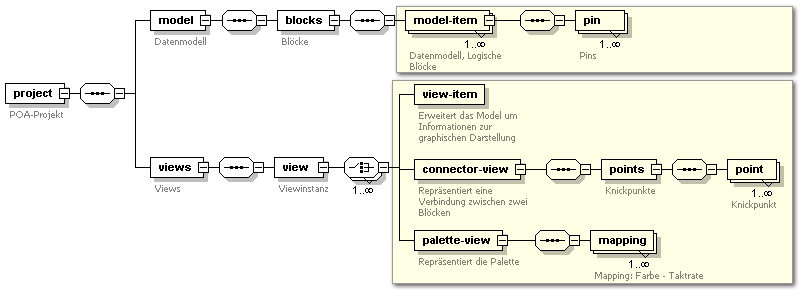
\includegraphics[width=17cm]{poa-schema.png}

\subsection{Struktur}
Die Projektdatei wird durch die folgenden Elemente strukturiert.

\begin{longtable}[c]{|p{5.466cm}|p{5.466cm}|p{5.466cm}|}
\hline
{\bf Element} & {\bf Unterelemente} & {\bf Beschreibung}\\\hline
\endhead
project      & model, view  & Wurzelelement \\\hline
model        & blocks       & Leitet den Modellbereich ein\\\hline
blocks       & model{}-item & Enth\"alt die Blockbeschreibungen\\\hline
model{}-item & pin          & Repr\"asentiert einen Block\\\hline
pin          &              & Repr\"asentiert einen Pin\\\hline
views        & view         & Leitet den Viewbereich ein\\\hline
view         & view{}-item, connector{}-view, palette{}-view &
Erweitert das Datenmodell um Darstellungsinformationen \\\hline

view{}-item  &              & Beschreibt die Position eines Blocks\\\hline
connector{}-view & points   & Beschreibt eine Verbindungslinie
zwischen zwei Bl\"ocken\\\hline

points & point & Enth\"alt die Knickpunkte der Verbindung\\\hline
point & & Repr\"asentiert einen Knickpunkt\\\hline
palette{}-view & mapping & Beschreibt die Position und die Eintr\"age
der Farbpalette \\\hline

mapping & & Verkn\"upft eine Taktfrequenz mit einer Farbe\\\hline
\end{longtable}


\subsection{Daten}
Die Projektdaten befinden sich in den Attributen der oben genannten Elemente.
\begin{longtable}[c]{|p{2.809cm}p{4.9420004cm}p{3.46cm}p{4.986cm}}
\hline
\multicolumn{1}{|p{2.809cm}|}{{\bf Element}} &
\multicolumn{1}{p{4.9420004cm}|}{{\bf Attribut}} &
\multicolumn{1}{p{3.46cm}|}{{\bf Datentyp}} &
\multicolumn{1}{p{4.986cm}|}{{\bf Beschreibung}}\\\hline
\endhead
model{}-item
&
\multicolumn{3}{p{13.788cm}}{\hspace*{-\tabcolsep}\begin{tabular}{|p{4.9420004cm}|p{3.46cm}|p{4.986cm}|}
id & int & Eindeutige Identifikation des Blocks\\\hline
name & String & Bezeichnung des Blocks\\\hline
desc & String & Beschreibung des Blocks in der Blockbibliothek\\\hline
hasOutputPins & boolean & Zeigt an, ob der Block Ausgangspins besitzt\\\hline
hasInputPins  & boolean & Zeigt an, ob der Block Eingangspins besitzt.\\\hline
hasEpisodicPins & boolean & Zeigt an, ob der Block episodische Pins
besitzt.\\\hline

clock & int & Taktrate des Blocks (ns)\\\hline
type  & String & Name der Rubrik unter der der Block in der
Blockbibliothek erscheint\\\hline
offset & int & Zeitlicher Versatz (ns)\\\hline
auto{}-offset & boolean & Zeigt an, ob der Versatz automatisch
berechnet wird\\\hline 

hasRuntime & boolean & Zeigt an, ob der Block eine Laufzeit besitzt.\\\hline
runtime & int & Laufzeit des Blocks (ns)\\\hline
block{}-type & \ {\quotedblbase}block``, {\quotedblbase}cpu`` &
Definiert den Typ des Blocks. {\quotedblbase}block`` repr\"asentiert
einen Core, {\quotedblbase}cpu`` eine CPU \\\hline
cpuid & int & Nummer der CPU auf dem CPLD \\\hline
\end{tabular}%\hspace*{-\tabcolsep}

}\\\cline{1-1}

pin&
\multicolumn{3}{p{13.788cm}}{\hspace*{-\tabcolsep}\begin{tabular}{|p{4.9420004cm}|p{3.46cm}|p{4.986cm}|}

id & int & Eindeutige Identifikation des Pins\\\hline
name & String & Bezeichnung des Pins\\\hline
address & int & Speicheradresse des Pins auf dem CPLD\\\hline
bits & int & Bitbreite des Pins\\\hline
type & {\quotedblbase}input``, {\quotedblbase}output``,
{\quotedblbase}episodic`` & Definiert um welche Art von Pin es sich
handelt\\\hline

position & int & Bestimmt die Reihenfolge der Pins am Block\\\hline
\end{tabular}\hspace*{-\tabcolsep}
}\\\cline{1-1}
\multicolumn{1}{|p{2.809cm}|}{
view

}&
\multicolumn{1}{p{4.9420004cm}|}{
name

}&
\multicolumn{1}{p{3.46cm}|}{
String

}&
\multicolumn{1}{p{4.986cm}|}{
Reserviert


}\\\hline

view{}-item


&
\multicolumn{3}{p{13.788cm}}{\hspace*{-\tabcolsep}\begin{tabular}{|p{4.9420004cm}|p{3.46cm}|p{4.986cm}|}


x, y & int & Position des Blocks auf dem Arbeitsbereich\\\hline
model{}-id & int & ID des {\textless}model{\textgreater}{}-Elements\\\hline
\end{tabular}\hspace*{-\tabcolsep}
}\\\cline{1-1}

connector{}-view


&
\multicolumn{3}{p{13.788cm}}{\hspace*{-\tabcolsep}\begin{tabular}{|p{4.9420004cm}|p{3.46cm}|p{4.986cm}|}


source{}-block, source{}-pin & int & Bestimmt Quell{}-Block und {}-Pin
f\"ur die Verbindung \"uber die jeweiligen Ids aus den
{\textless}model{\textgreater}{}-Elementen\\\hline

target{}-block, target{}-pin & int & Bestimmt Ziel{}-Block und {}-Pin
f\"ur die Verbindung \"uber die jeweiligen Ids aus den
{\textless}model{\textgreater}{}-Elementen\\\hline
\end{tabular}\hspace*{-\tabcolsep}
}\\\cline{1-1}
\multicolumn{1}{|p{2.809cm}|}{
point


}&
\multicolumn{1}{p{4.9420004cm}|}{
x, y


}&
\multicolumn{1}{p{3.46cm}|}{
int


}&
\multicolumn{1}{p{4.986cm}|}{
Position des Knickpunkts auf dem Arbeitsbereich


}\\\hline

palette{}-view


&
\multicolumn{3}{p{13.788cm}}{\hspace*{-\tabcolsep}\begin{tabular}{|p{4.9420004cm}|p{3.46cm}|p{4.986cm}|}


x, y & int & Position der Palette auf dem Arbeitsbereich\\\hline
last{}-pal{}-entry & int & Definiert die Index{}-Nummer auf der
Farbpalette, die f\"ur die n\"achste Taktrate verwendet werden soll\\\hline

name & String & Bezeichner der Palette (reserviert)\\\hline
\end{tabular}\hspace*{-\tabcolsep}
}\\\cline{1-1}

mapping &
\multicolumn{3}{p{13.788cm}}{\hspace*{-\tabcolsep}\begin{tabular}{|p{4.9420004cm}|p{3.46cm}|p{4.986cm}|}

ns & int & Taktfrequenz in Nanosekunden.\\\hline

pal{}-entry & int & Index{}-Nummer auf der Farbpalette.\\\hline
\end{tabular}\hspace*{-\tabcolsep}
}\\\cline{1-1}
\end{longtable}

\subsection{Document Type Definition}

\lstset{
  language=XML, %The programminglanguage to be used
  basicstyle=\scriptsize\ttfamily, %The text size of the code
  keywordstyle=\color{red}\bfseries,
  commentstyle=\color{blue}, % blue comments
  showspaces=false, %Leaves spaces blank
  showstringspaces=false, %Leaves spaces in strings blank
  breaklines=true, %Break lines that are too long
  fontadjust=true,
  extendedchars=false, %Includes danish charactors
  numbers = left, %Shows linenumbers
  stepnumber = 1 %The interval with which linenumbers are displayed
}
\begin{lstlisting}{language=XML}
<?xml version="1.0" encoding="UTF-8"?>
<!-- root element -->
<!ELEMENT project (model, views)>

<!-- model elements -->
<!ELEMENT model (blocks)>
<!ELEMENT blocks (model-item+)>
<!ELEMENT model-item (pin+)>
<!ATTLIST model-item
	offset CDATA #REQUIRED
	desc CDATA #REQUIRED
	hasOutputPins CDATA #REQUIRED
	hasInputPins CDATA #REQUIRED
	clock CDATA #REQUIRED
	runtime CDATA #REQUIRED
	hasEpisodicPins CDATA #REQUIRED
	type CDATA #REQUIRED
	id CDATA #REQUIRED
	name CDATA #REQUIRED
	auto-offset CDATA #REQUIRED
	hasRuntime CDATA #REQUIRED
	block-type (block | cpu) #REQUIRED
	cpuid CDATA #IMPLIED
	auto-runtime CDATA #IMPLIED
>
<!ELEMENT pin EMPTY>
<!ATTLIST pin
	address CDATA #REQUIRED
	bits CDATA #REQUIRED
	position CDATA #REQUIRED
	type (input | output | episodic) #REQUIRED
	id CDATA #REQUIRED
	name CDATA #REQUIRED
>

<!-- view elements -->
<!ELEMENT views (view)>
<!ELEMENT view (view-item | connector-view | palette-view)+>
<!ATTLIST view
	name CDATA #REQUIRED
>
<!ELEMENT view-item EMPTY>
<!ATTLIST view-item
	x CDATA #REQUIRED
	y CDATA #REQUIRED
	model-id CDATA #REQUIRED
>

<!-- connectors -->
<!ELEMENT connector-view (points)>
<!ATTLIST connector-view
	target-pin CDATA #REQUIRED
	target-block CDATA #REQUIRED
	source-pin CDATA #REQUIRED
	source-block CDATA #REQUIRED
>
<!ELEMENT points (point+)>
<!ELEMENT point EMPTY>
<!ATTLIST point
	x CDATA #REQUIRED
	y CDATA #REQUIRED
>

<!-- palette -->
<!ELEMENT palette-view (mapping+)>
<!ATTLIST palette-view
	last-pal-entry CDATA #REQUIRED
	x CDATA #REQUIRED
	y CDATA #REQUIRED
	name CDATA #REQUIRED
>
<!ELEMENT mapping EMPTY>
<!ATTLIST mapping
	ns CDATA #REQUIRED
	pal-entry CDATA #REQUIRED
>
\end{lstlisting}